\chapter{Beschreibung des Versuchs}

Der Laborversuch besch�ftigt sich mit einer Einf�hrung in die Konfiguration von
IPv6 \acp{LAN}.

\section{Versuchsaufbau}\label{Aufbau}

\begin{figure}[ht]
  \centering
     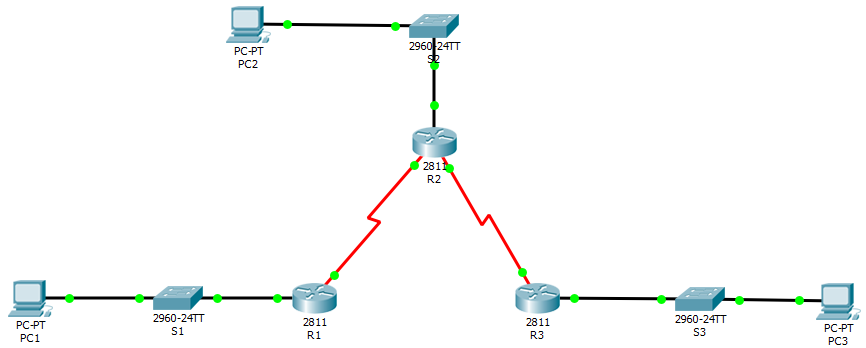
\includegraphics[width=\linewidth]{Graphics/aufbau.PNG}
  \caption{Versuchsaufbau}
  \label{fig:aufbau}
\end{figure}


\subsection{Komponenten}

\begin{itemize}
  	\item 3 Computer
  	\item 3 Cisco 2811 Router
  	\begin{itemize}
      	\item Verbindung zum jewiligen Switch durch Straight-Through-Kabel
      	\item Verbindung zwischen Router 1 und Router 2 durch Serial-Kabel
      	\item Verbindung zwischen Router 2 und Router 3 durch Serial-Kabel
	\end{itemize}
  	\item 3 Cisco 2960 Switches
  		\begin{itemize}
    	\item Verbindung zum jewiligen Host durch Straight-Through-Kabel
   		\end{itemize}
\end{itemize}

\clearpage

\section{Versuchsdurchf�hrung}

Aus organisatorischen Gr�nden wurde dieser Laborversuch mittels
Cisco PacketTracer durchgef�hrt.

\begin{table}[!htbp]
\centering
\small
	\begin{tabularx}{1.05\textwidth}{|X|X|X|X|}
	\hline
	\textbf{Device} & \textbf{Interface} & \textbf{IPv6-Address/Prefix} & \textbf{Default Gateway} \\
	\hline
	R1 & F0/0 & 2001:DB8:1:1::1/64 & N/A \\
	\hline
	R1 & S0/0/0 (DCE) & 2001:DB8:1:A001::1/64 & N/A \\
	\hline
	R1 & Link-local & FE80::1 & N/A \\
	\hline
	R2 & F0/0 & 2001:DB8:1:2::1/64 & N/A \\
	\hline
	R2 & S0/0/0 & 2001:DB8:1:A001::2/64 & N/A \\
	\hline
	R2 & S0/0/1 (DCE) & 2001:DB8:1:A002::1/64 & N/A \\
	\hline
	R2 & Link-local & FE80::2 & N/A \\
	\hline
	R3 & F0/0 & 2001:DB8:1:3::1/64 & N/A \\
	\hline
	R3 & S0/0/1 & 2001:DB8:1:A002::2/64 & N/A \\
	\hline
	R3 & Link-local & FE80::3 & N/A \\
	\hline
	PC1 & NIC & 2001:DB8:1:1::F/64 & FE80::1 \\
	\hline
	PC2 & NIC & 2001:DB8:1:2::F/64 & FE80::2 \\
	\hline
	PC3 & NIC & 2001:DB8:1:3::F/64 & FE80::3 \\
	\hline
	\end{tabularx}
\caption{Konfiguration}
\label{config1}
\end{table}
%TODO Tabelle vervollst�ndigen
\underline{Weiteres Vorgehen:}
\begin{itemize}
  \item Konfiguration der Router
  \item Konfiguration der Hosts
  \item IPv6-Routen konfigurieren
\end{itemize}

\section{Versuchsziel}
